\documentclass[12pt, a4paper]{article}

\usepackage[utf8]{inputenc}
\usepackage{graphicx} % to embed images
\usepackage{rotating}
\usepackage{hyperref} % to link the table of contents
\usepackage{subcaption} %complex images
\usepackage{placeins} %floating
\usepackage{pdflscape} %to allow single pages in landscape mode
\usepackage[top=1.25in, bottom=1.25in, left=1in, right=1in]{geometry}
\usepackage{verbatim} % include raw text file (for Alloy)
\usepackage[ruled, vlined]{algorithm2e} % algorithms
\usepackage[export]{adjustbox}

\title{Design Document}
\date{2016-12-11}
\author{
	Patricia Abbud
	\and
	Maddalena Andreoli Andreoni
	\and
	Paolo Cudrano
}

\begin{document}
	%%% titlepage %%%
	\begin{titlepage}
		\centering
		
\includegraphics[width=5cm]{img/polimi_logo.png} % also works with logo.pdf
		\vfill
		{\bfseries\Large
			PowerEnJoy\\
			Design Document\\
			Version 2
			\vskip4cm
			Patricia Abbud\\
			Maddalena Andreoli Andreoni\\
			Paolo Cudrano\\
		}
		\vfill
		\vfill
	\end{titlepage}

	%%% table of contents %%%
	\tableofcontents
	\newpage

	\section{Introduction}
		\subsection{Purpose}
This Design Document describes the architecture and design choices for \textit{PowerEnJoy}'s system the team is to develop. The document will be divided in five main chapters (aside from the introduction and appendixes): the \textbf{Architectural Design} chapter will describe in detail our system, the architectural choices we made and its design. It will make use of UML diagrams as well as text descriptions, going from a high-level view to a more deep and in-detail analysis. The \textbf{Algorithm Design} will focus on the most relevant algorithmic parts of the system, mainly related to the \textit{money saving option}: it will contain a short description of each algorithm as well as the algorithm itself. 
The \textbf{User Interface Design} section will provide an overview of the user interfaces of the system. Since some of it have already been described in the RASD document, this section will only contain the remaining ones. 
Finally, the \textbf{Requirements Traceability} will map the requirements defined in the RASD document to the design elements defined in this document.
Every step in the decision process will be documented and explained.

\subsection{Scope}
The goal of this project is to create \textit{ex novo} a system for the car-sharing service \textit{PowerEnJoy}. This system will provide users throughout the city an easy and user-friendly way to reserve and drive electric cars, and also to interact with the company's operators and administrators in the eventuality of a break down or an accident.

\subsection{Definitions, acronyms, abbreviations}
% TODO

\subsection{Reference documents}
% TODO

\subsection{Document structure}
% TODO

	\newpage
	\section{Architectural design}
		\subsection{Overview}
			The system is structured on a \textbf{three-tier architecture}, with tiers divided as follows.
\begin{itemize}
	\item{Clients.} The system can be accessed from several applications running on different categories of devices, each of them providing a specific subset of functionalities. In particular:
	\begin{itemize}
		\item{User web browser.} A website, mainly used as showcase, provides a section for the management of registration and the visualization of already registered accounts.
		\item{User mobie app.} A mobile application allows registered users to employ the services provided by \textit{PowerEnJoy}.
		\item{Car client.} The cars run a custom application on their on-board tablet to inform the users and interact with them about the ride in progress. This application is also responsible to keep the car connected to the rest of the system.
		\item{Operator mobile app.} Every operator is equipped with a mobile device running a custom application. This application allows them to perform their assistance tasks and keep the connection with the administrators.
		\item{Admin app.} The administrators can control the system parameters and manage the operators dispatching by means of a specific application running on their desktop devices.
	\end{itemize}
	\item{App server.} A business logic server is designed to expose services to the clients. It is placed inside a DMZ to guarantee a higher degree of security.
	\item{Database server.} All the relevant data for the system are stored on a designated server, protected by a double layer of firewalls from outside attacks.
\end{itemize}
To this structure, an addition is made to fulfill all the requirements:
	\begin{itemize}
		\item{Web server.} A specific server is used to store the website static pages, becoming a parallel tier with respect to the app server.
	\end{itemize}

\begin{figure}[h]
	\includegraphics[width=350pt, center]{img/tiers.png} % FIXME labels in image\\
	\caption{Three-tier architecture}
\end{figure}
\FloatBarrier

\subsubsection{Layers vs Tiers}
	From a logical point of view, the clients mentioned above provide significantly different functionalities. For this reason, the allocation of the layers (Presentation, Application and Data) to these three tiers becomes dependent on the nature of the client involved in this process.

	\paragraph{User web browser, Admin app.} These applications provide a very limited set of functionalities, relieving them from the need of logical computation client-side. For this reason, the clients provide only the presentation, whereas the application layer is entirely managed by the application server. Finally, the database server is left responsible for the data layer.
		\begin{figure}[h]
			\includegraphics[width=250pt, center]{img/tier_layer_mapping_thinclient.png}
			\caption{Layers allocation in clients: User web browser, Admin app}
		\end{figure}

	\paragraph{User mobile app, Car client, Operator mobile app.} For these applications, responsible for more complex functionalities, it is necessary to delegate part of the computations to the clients. Therefore, in this case the application layer is divided between the client app and the application server. As for the others, the presentation layer is assigned to the clients, while the data are managed by the database server.
		\begin{figure}[h]
			\includegraphics[width=250pt, center]{img/tier_layer_mapping.png}
			\caption{Layers allocation in clients: User mobile app, Car client, Operator mobile app}
		\end{figure}
\FloatBarrier


		\subsection{Component view}
			The Component Diagram shown below describes the logical components of the system we are to develop, from a very high-level description on to a more detailed one. This diagram does not take into account the deployment phase, hence it doesn't describe the logical layer of the system in terms of the physical tiers where it is deployed. It also does not show the interfaces between the logical layer and the end users or the database, for simplicity and readability. 


	\subsubsection{High level components}
		\paragraph{} We shall show below the high level view of the logical components of the system and their interactions. Following the UML 1 notation, the dashed arrows represent dependencies between components, with the tail end component depending on the point end component (e.g. if \textit{A $\rightarrow$ B}, then A \textit{depends on} B). 

		
		\begin{figure}[h]
			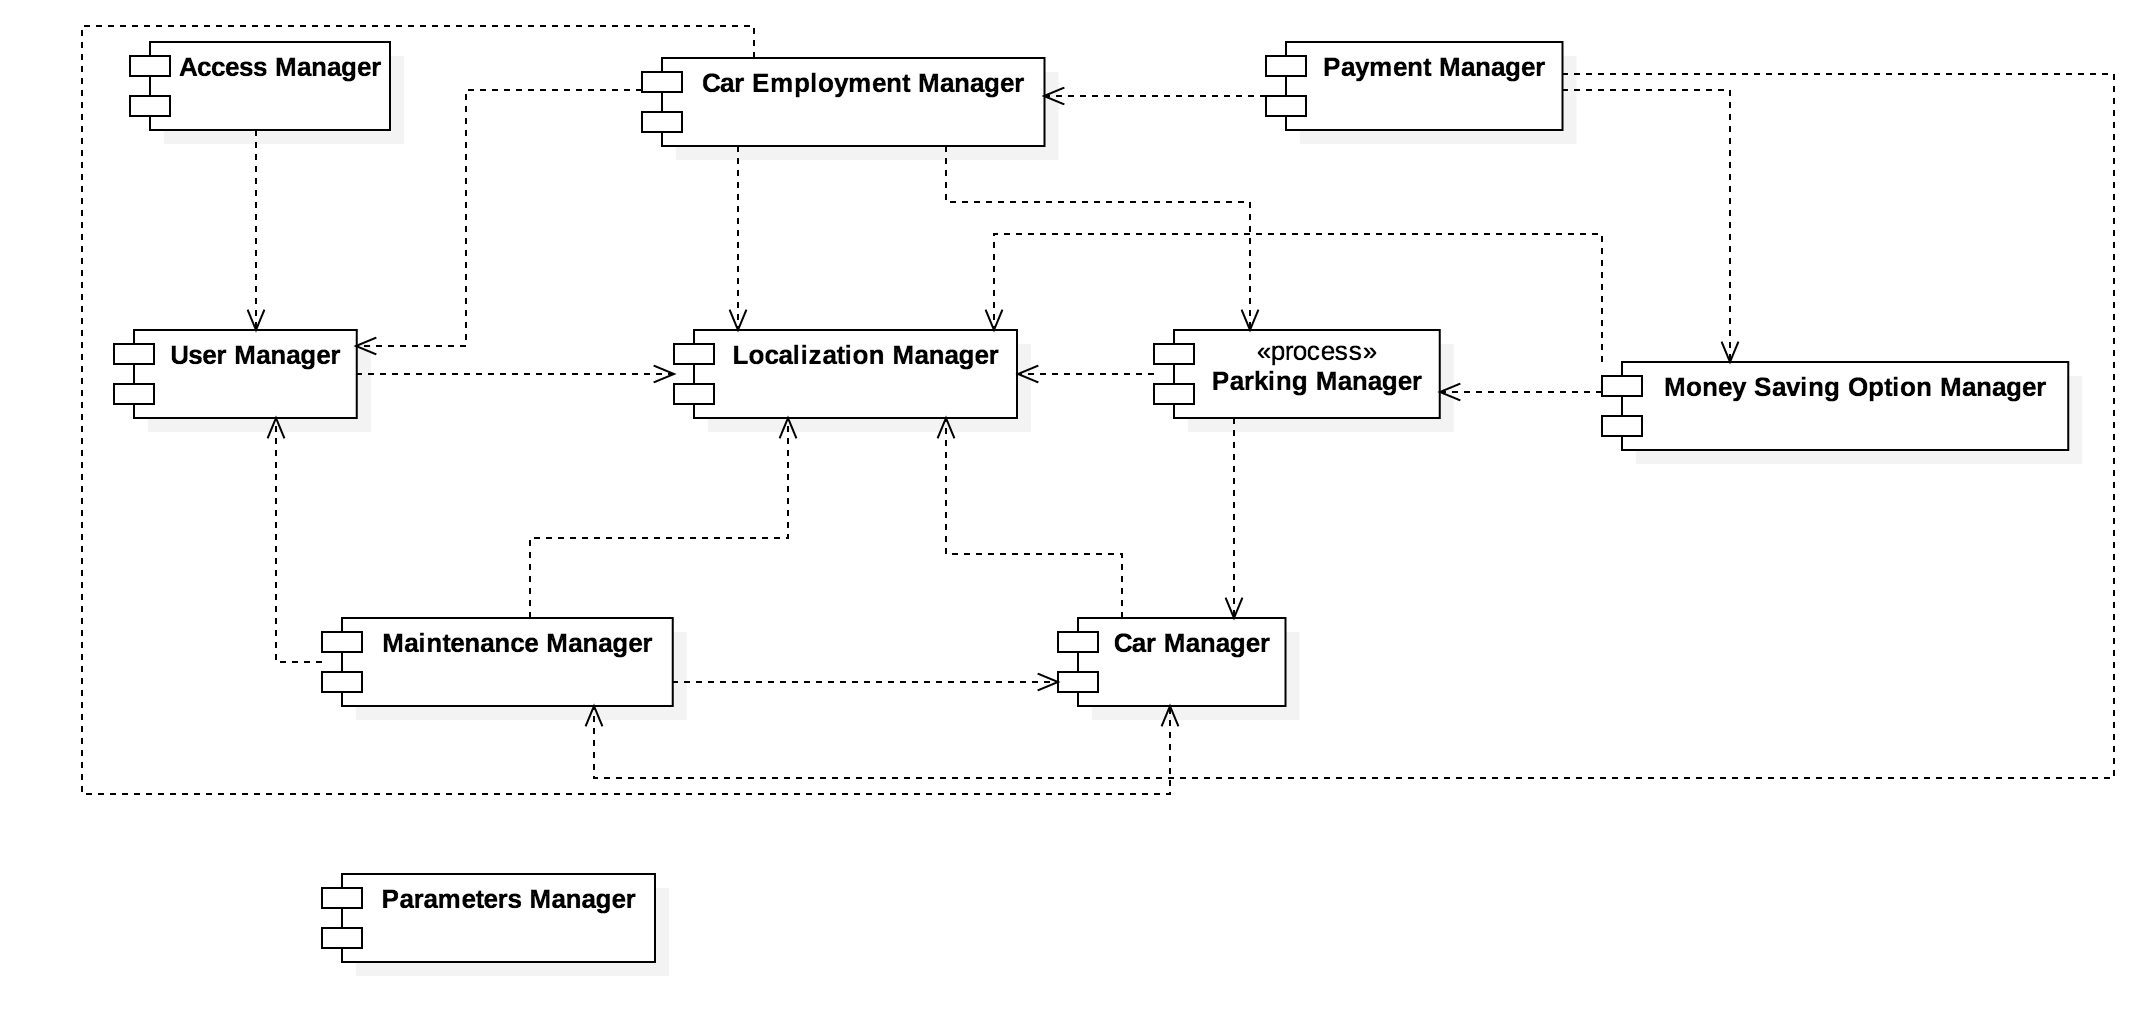
\includegraphics[scale=0.26, center]{img/component_diagrams/01_high_level_component_view.png}
			\caption{High level view}
		\end{figure}
\FloatBarrier


	\subsubsection{Component view}
	
	%\paragraph{Access Manager}
	\subsubsection*{Access Manager}
		
		
			
			
		\paragraph{}The Access Manager deals with the first interactions of a user or a guest with the system at the beginning of each session. Every further interaction with the system requires either a log in or the registration, both of which are managed by independent processes. The login interfaces with the User Handler to verify the validity of the login information and to allow the authenticated user to continue employing the system. Both processes also interface with the database.

		\begin{figure}[h]
				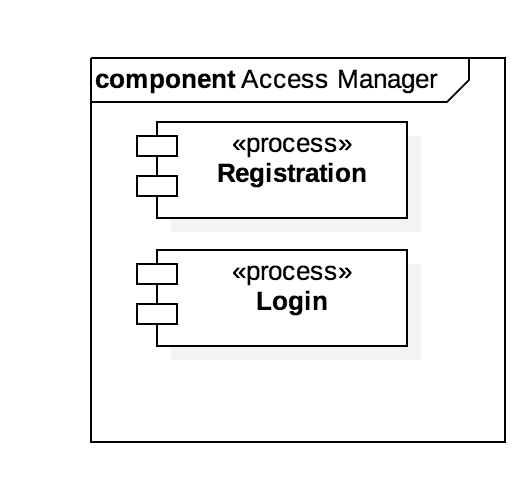
\includegraphics[scale=0.4, center]{img/component_diagrams/02_access_manager.png}
				\caption{Component Access Manager}
			\end{figure}
		
\FloatBarrier		
		
		\subsubsection*{User Manager}
		
		
		
		
		\paragraph{} The User Manager manages all interaction that a registered user has with the rest of the system. The User Handler functions as an interface component between the user themselves and the system, and to be associated with a user needs to be linked to the Profile Manager. This latter component interfaces with the DBMS and controls the validity of all data in the user's profile and its changes; the exception to this is the driving license data, that is checked by the License Manager since it's a particularly critical piece of information. The Profile Manager also depends on the License Manager in that every time the user tries to reserve a car the Profile Manager asks the License Manager for the validity of the user's license. 
		\begin{figure}[h]
			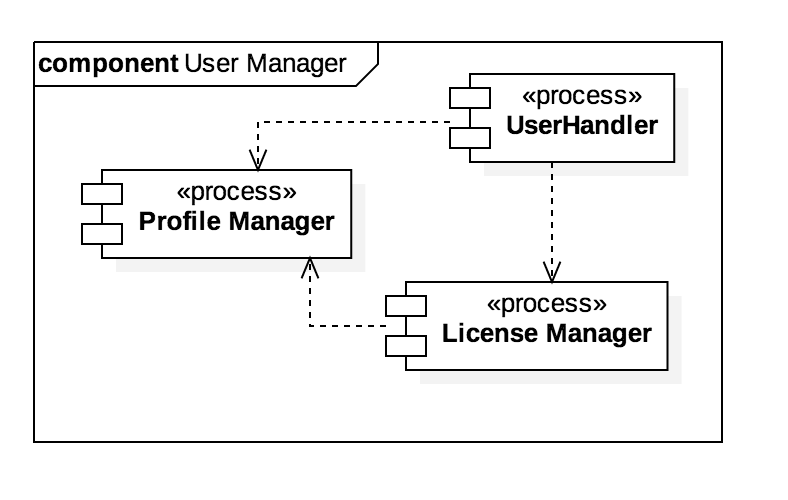
\includegraphics[scale=0.4, center]{img/component_diagrams/03_user_manager.png}
			\caption{Component User Manager}
		\end{figure}	
\FloatBarrier

		
		
		\subsubsection*{Car Employment Manager}
		
			
			
		\paragraph{} The Car Employment Manager is one of the most important component of the system in terms of its core functionalities. It's composed of three processes: the first one, the Reservation Handler, has the task of dealing with reservations from a user and for an individual car. It blocks all other possible operations to that car until the user starts using it or the reservation expires. To keep track of the time, the Reservation Handler needs to interface with the Time Manager. This process is tasked with keeping track of the time periods necessary for the services to be offered: the expiration time for a reservation, the duration of a ride, the time window after a ride has finished. 
		The Ride Handler on the other hand depends on the Reservation Handler in that a car can be used only after a reservation. The Ride Handler is associated to a particular car and a particular user. It depends on the Time Manager to keep track of the duration of the ride. 
		\begin{figure}[h]
			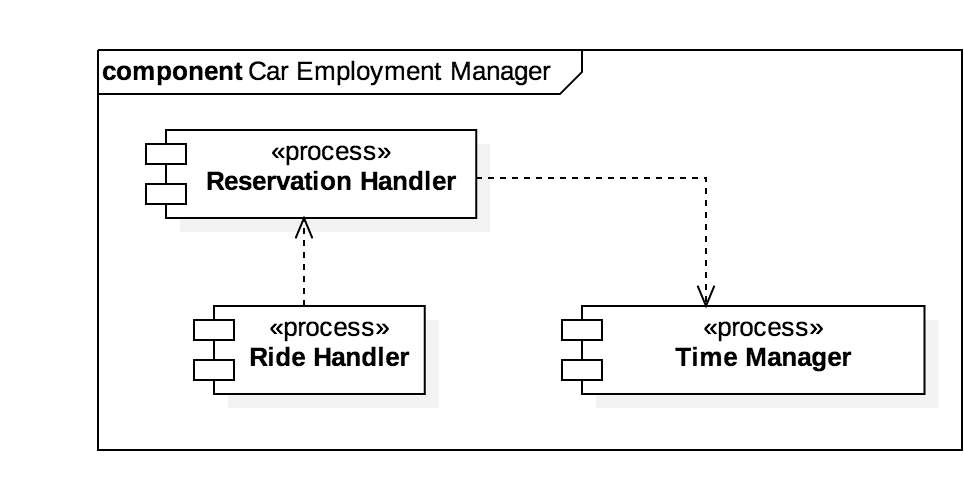
\includegraphics[scale=0.4, center]{img/component_diagrams/04_car_employment_manager.png} %TODO modify the image, a dependency is missing
			\caption{Component Car Employment Manager}
		\end{figure}	
\FloatBarrier

		
		
		\subsubsection*{Localization Manager}
		
		
			
		\paragraph{} The Localization Manager handles all the localization issues of the system. Its three components, the User Location Handler, the Car Location Handler and the Operator Location Handler (that track, respectively, users, cars and operators) all work independently from each other and interface with the respective handlers from other components. The Localization Manager also interfaces with the external Map Services Provider, that provides the information for the localization.
		\begin{figure}[h]
			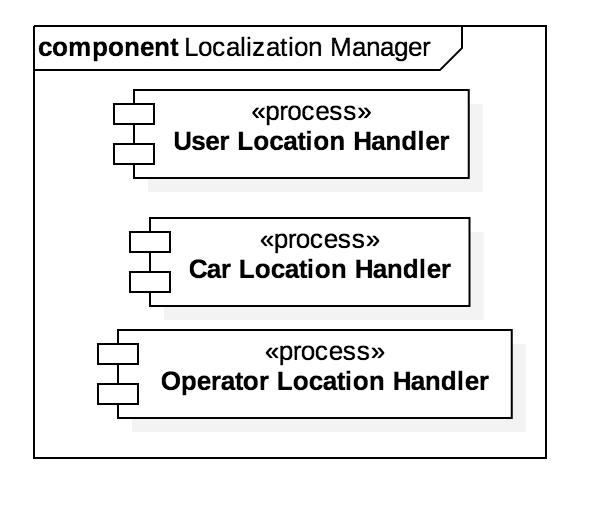
\includegraphics[scale=0.4, center]{img/component_diagrams/05_localization_manager.png}
			\caption{Component Localization Manager}
		\end{figure}	
\FloatBarrier		
		
		
		\subsubsection*{Maintenance Manager}
		
		
		\paragraph{} The Maintenance Manager deals with emergencies and daily maintenance of the cars. For this purpose, it has an interface with the operators, the Operator Handler; the operators are dispatched by the admins and are associated to some emergency report. The Dispatcher Manager handles the availability and the tasks associated with each operator; the Emergency Report Handler on the other hand manages the emergency reports, associating them with a user, a car and an operator, and keeping track of their status thanks to the Report Status Handler.
		\begin{figure}[h]
			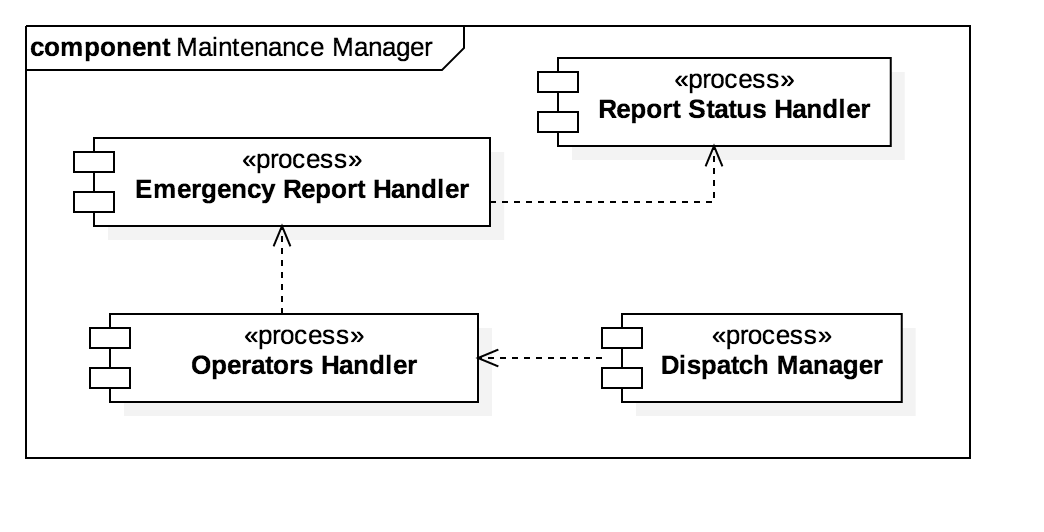
\includegraphics[scale=0.4, center]{img/component_diagrams/06_maintenance_manager.png}
			\caption{Component Maintenance Manager}
		\end{figure}	
		

\FloatBarrier		
		
		
		
		\subsubsection*{Backend Manager}
			
			
		\paragraph{} The Backend Manager oversees all operations entrusted to the administrators. The Admin Handler is the interface between the admins and the system, and keeps track of each administrator's activities and identification. The Parameters Manager deals with all changes done to the parameters of the system (their validity within fixed boundaries, their actual deployment); it depends on the Admin Handler since every change to the parameters is done by an admin. %FIXIT actual deployment??
		\begin{figure}[h]
				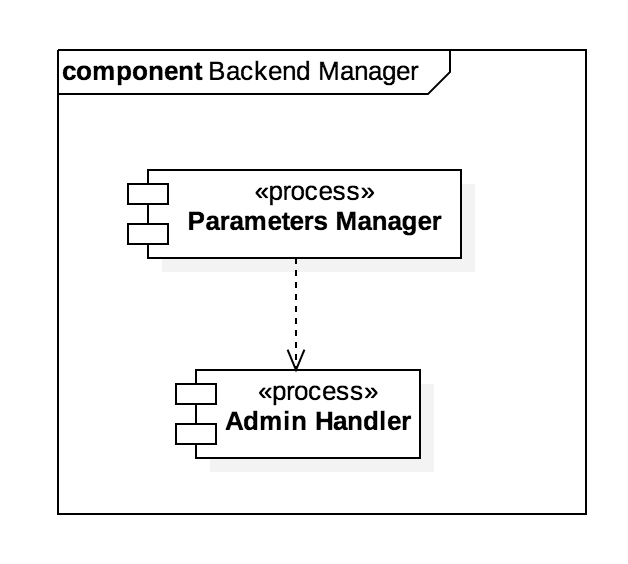
\includegraphics[scale=0.4, center]{img/component_diagrams/11_backend_manager.png}
				\caption{Component Backend Manager}
			\end{figure}
\FloatBarrier
	
		
		
		
		\subsubsection*{Car Manager}
			
		
		\paragraph{} The Car Manager interfaces the car with the rest of the system. The Sensors Manager gathers and parses the raw signals provided by all the sensors in the car. It also is the direct line of communication between the car and the Car Handler. The Car Handler interprets the information provided by the Sensors Manager and acts upon it, notifying other components or giving commands to the sensors.
		 \begin{figure}[h]
				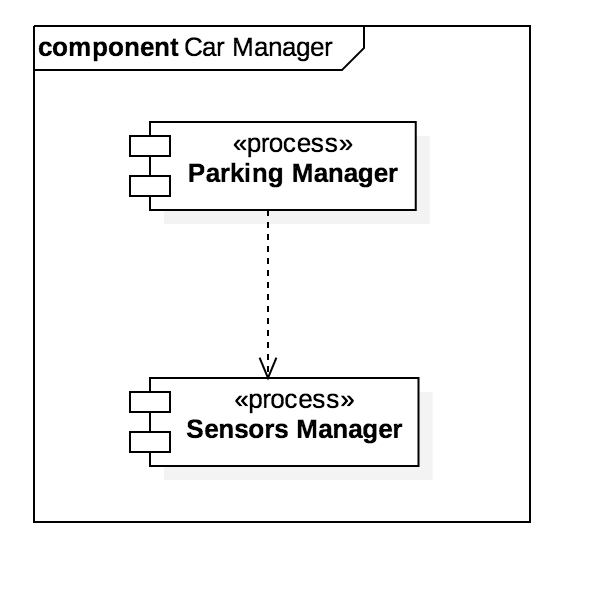
\includegraphics[scale=0.4, center]{img/component_diagrams/07_car_manager.png}
				\caption{Component Car Manager}
			\end{figure}
\FloatBarrier
		
		
		
		
		\subsubsection*{Payment Manager}
			
			
		\paragraph{} Through the Payment Manager, the system keeps track of the fare of each ride and the extraordinary fees (i.e. the fines), the discounts and the sanctions to charge the user. The Payment Handler is arguably the most important process since it's the one that is tasked with keeping track of the total cost for a ride. To do that, it needs to interface with the Ride Handler, and also with the Discounts and Sanctions Handler, to be able to consider them in its calculations. The Exceptional Payment Handler manages the exceptional fees, such as fines for expired reservations or for damages to the car. All of them are needed by the Invoice Manager, that takes the final charge from them and notifies the external Payment Services Provider, such that it may invoice the user of their charges.
		\begin{figure}[h]
				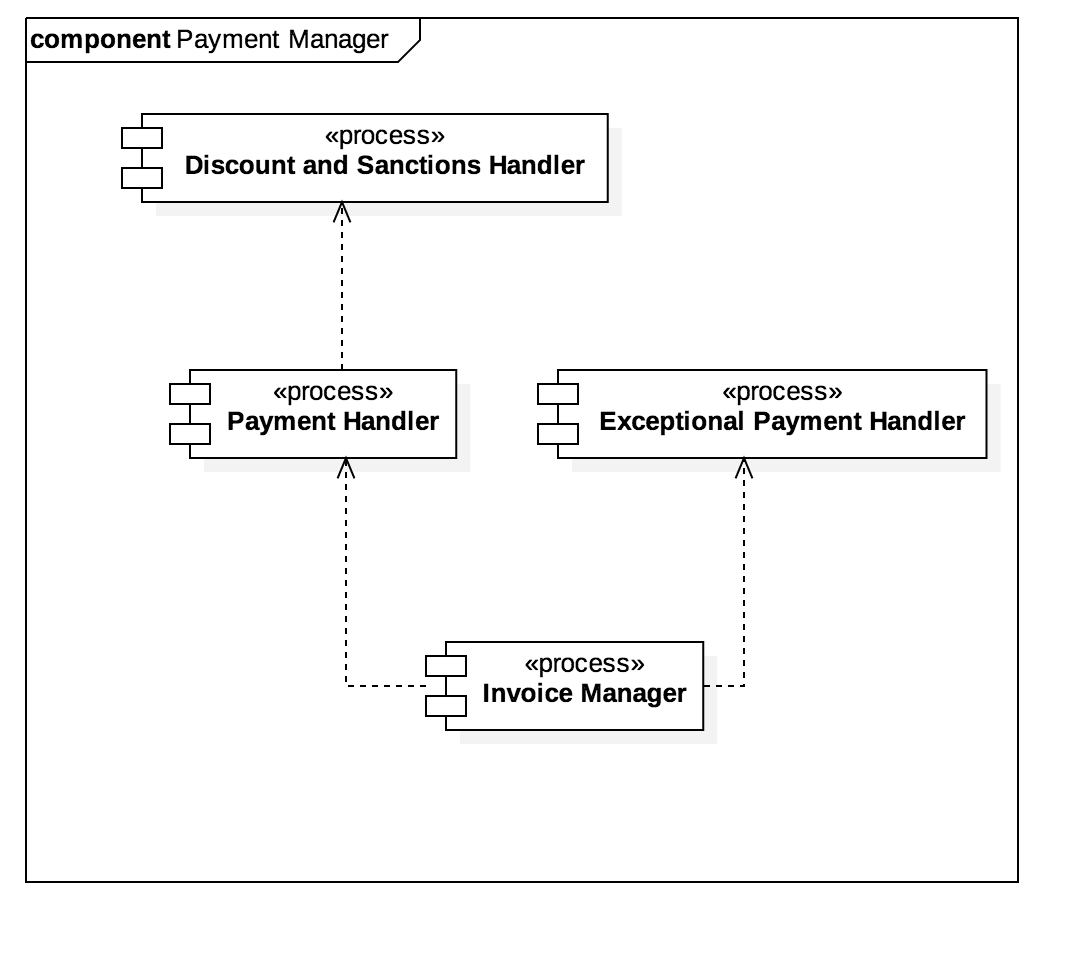
\includegraphics[scale=0.4, center]{img/component_diagrams/08_payment_manager.png}
				\caption{Component Payment Manager}
			\end{figure}
\FloatBarrier	
		
		
		
		\subsubsection*{Money Saving Option Manager}
			
		
		\paragraph{} We decided to dedicate an entire component for the sole purpose of managing the Money Saving Option (MSO), because of its complexity. The Discounts and Sanctions Handler also depends on this component to provide the information on whether to apply the relative discount or not. It has two processes, which are the Parking Distribution Handler and the MSO Handler. The Parking Distribution Handler takes the brunt of the computing complexity since its task is to calculate the optimal distribution of cars with an heuristic algorithm. On the other hand, the MSO Handler gets the necessary information from the Parking Distribution Handler and decides which Parking Area to notify the user given the destination of the ride.
		%FIXIT TMI?
		\begin{figure}[h]
				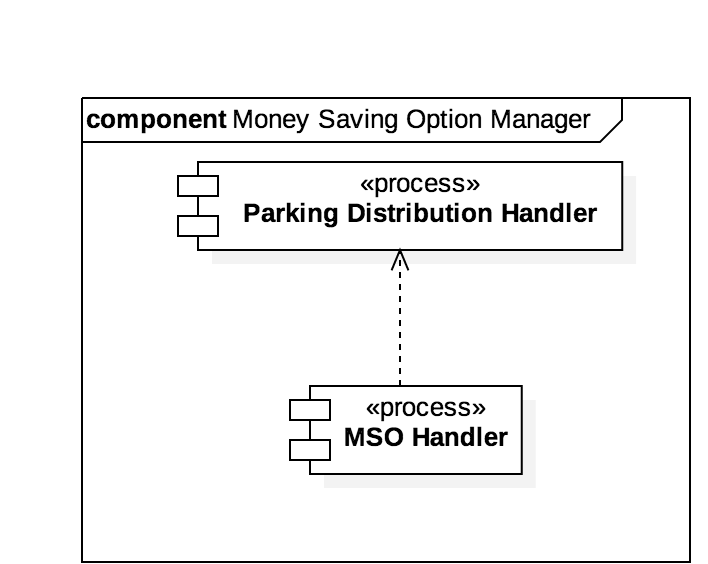
\includegraphics[scale=0.4, center]{img/component_diagrams/09_money_saving_option_manager.png}
				\caption{Component Money Saving Option Manager}
			\end{figure}
\FloatBarrier		
		
		\subsubsection*{Parking Manager}
		
			%FIXIT no image? do we need it?
		
		\paragraph{} The Parking Manager keeps tabs on where (and if) a car is parked, and for how long. Thanks to the Car Location Manager and the Car Sensors, it locates cars and decides whether they are parked inside a Safe Area or not; it also depends on the Time Manager to calculate the window of time after the end of a ride when a user is still allowed to plug the car into the power grid or open it.
		%FIXIT change direction of arrow between time manager and parking manager?
\FloatBarrier

	\subsubsection{Complete component view}
	
	The following figure shows the complete component diagram for the system, with all the dependencies as shown. 
	
		\begin{sidewaysfigure}
			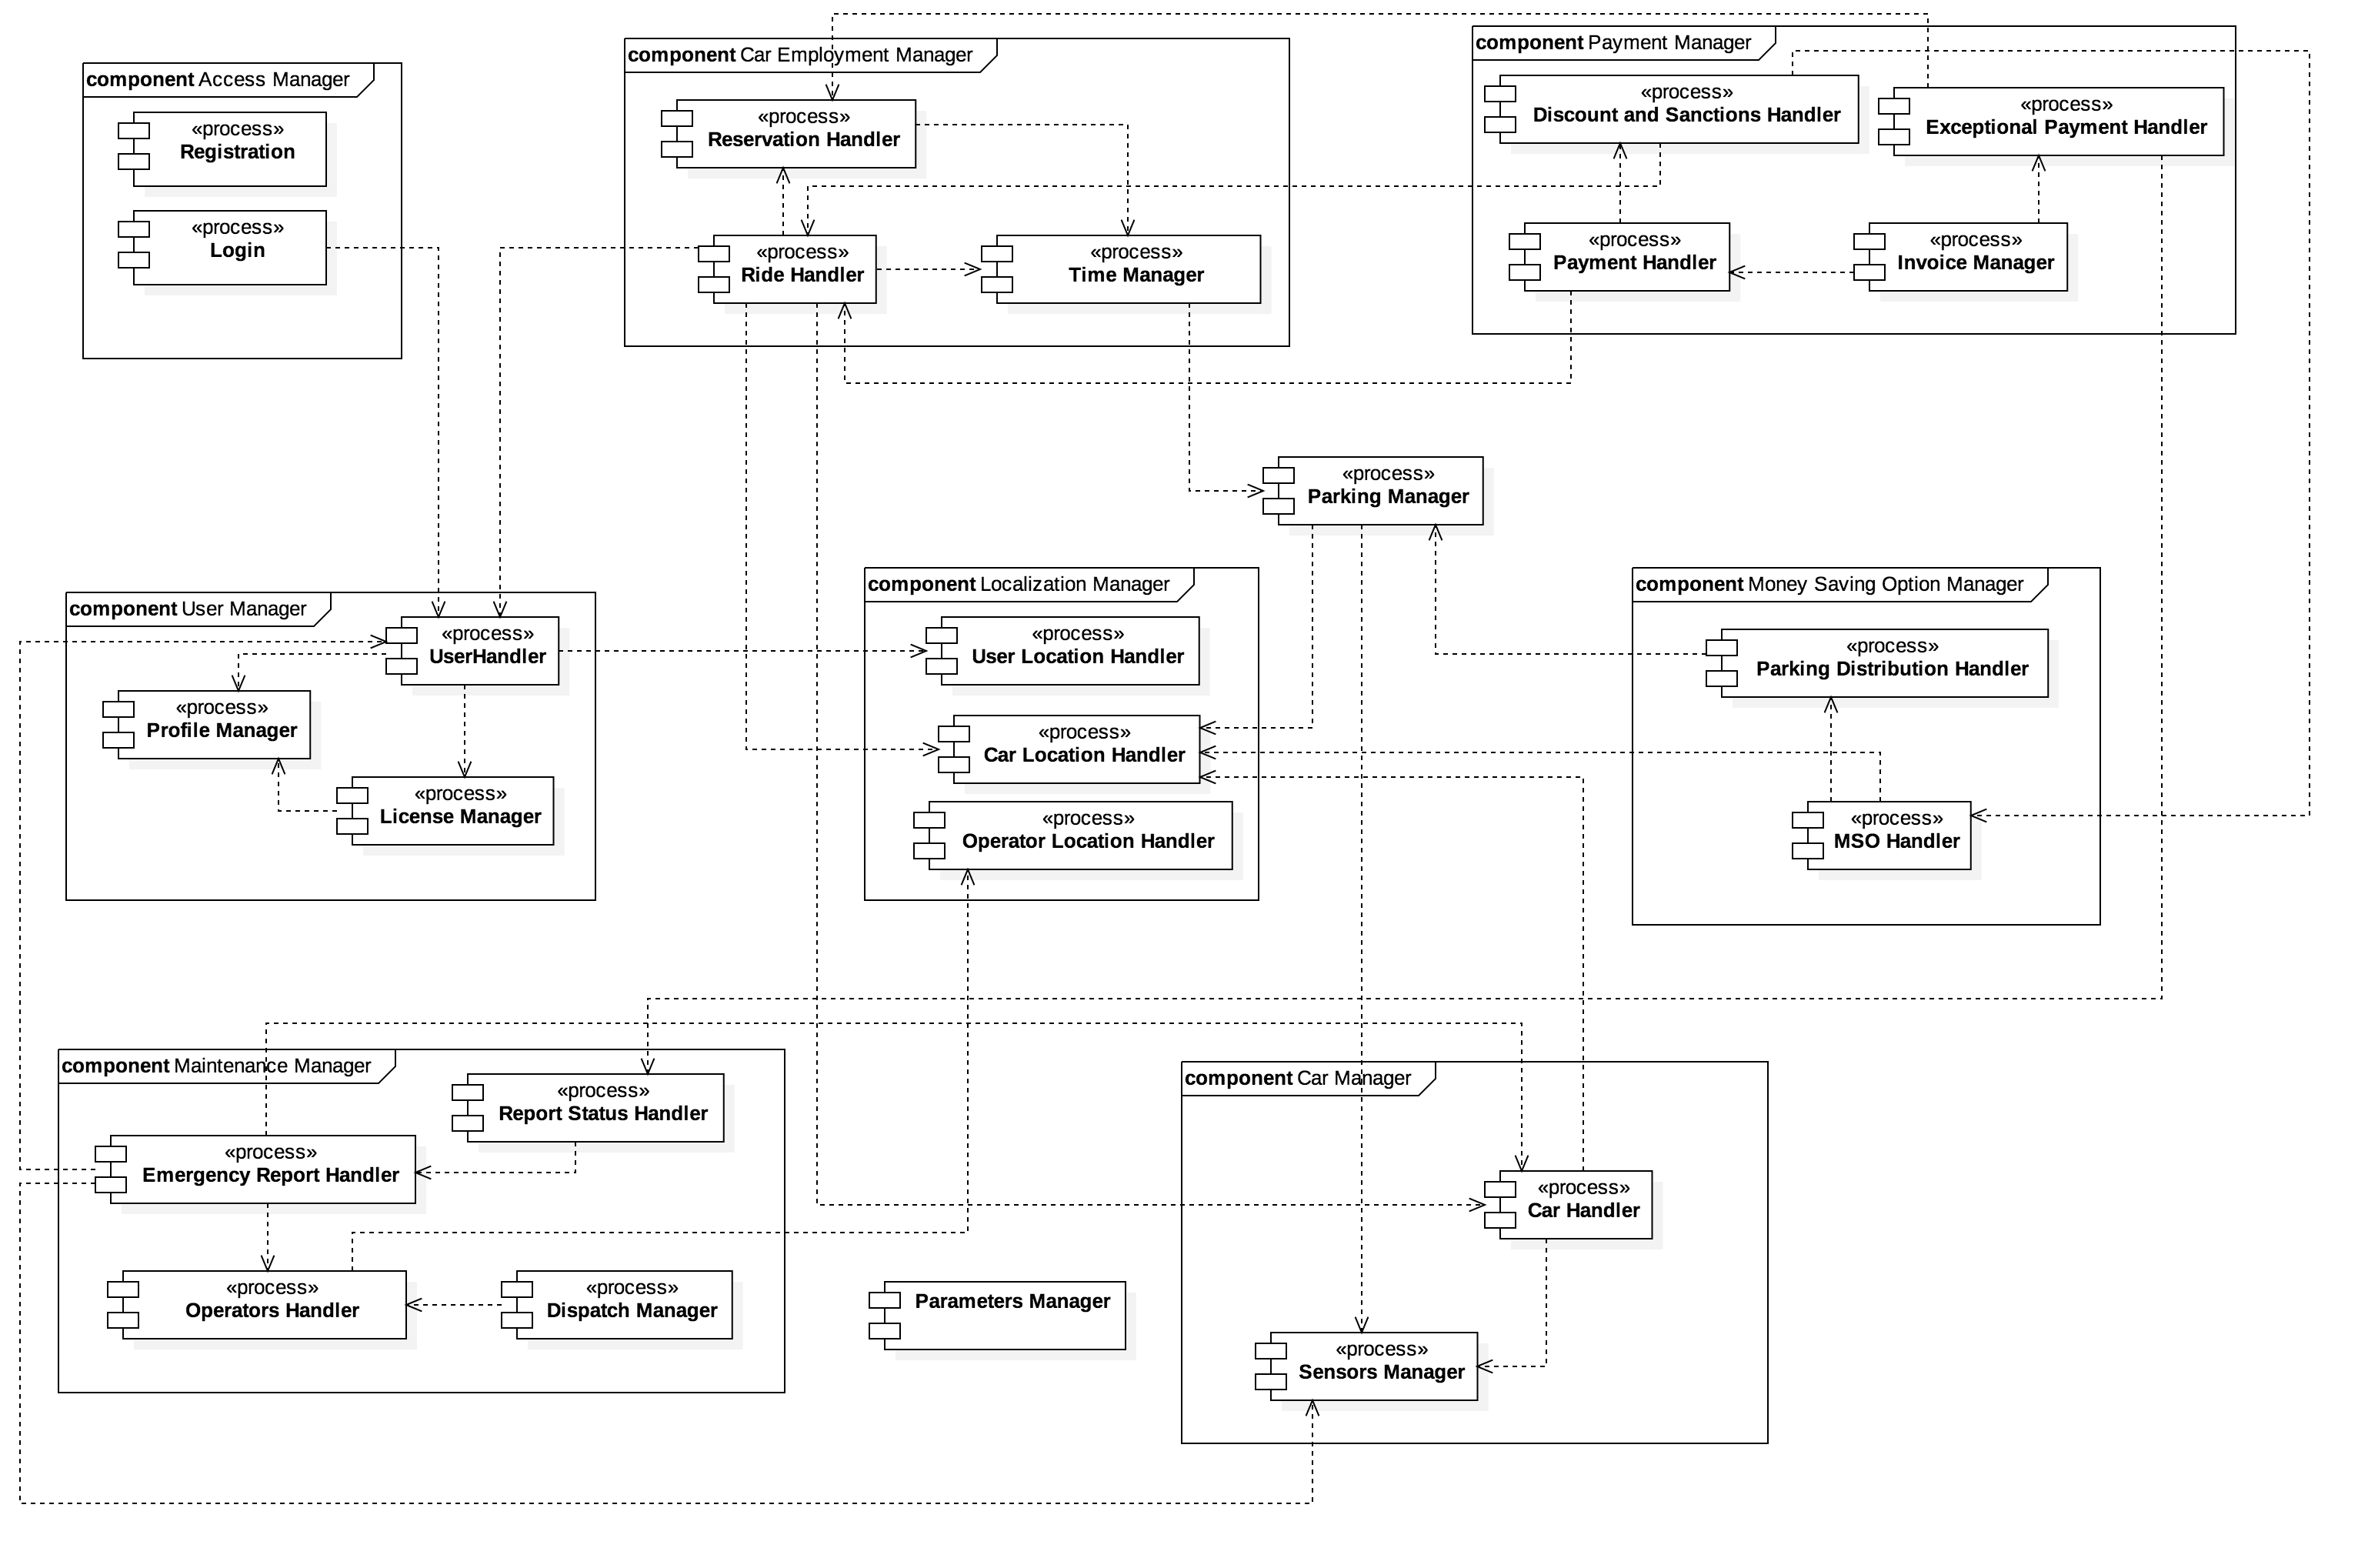
\includegraphics[width=\hsize, center]{img/component_diagrams/10_complete_component_view.png}
			\caption{Complete Component View}
		\end{sidewaysfigure}
			
\FloatBarrier


		\subsection{Deployment view}
			The Deployment Diagram shown below describes how the logical components designed in the context of the Component Diagram are to be physically deployed on the different devices needed for the functioning of the system.

As shown, the app server hosts the main logic components and manages their interaction. It provides access to them through the APIs defined in \autoref{sec:components_interfaces} and guarantees they can access the data layer residing on the database server.\newline
Every client with a significant application layer implements a limited subset of components responsible to interpret the inputs from the users and perform requests to the app server. When needed, an apposite module for the localization is included as well.\newline
The web server provides static web pages and the logic necessary to the browser to interact with the app server.

\begin{sidewaysfigure}
	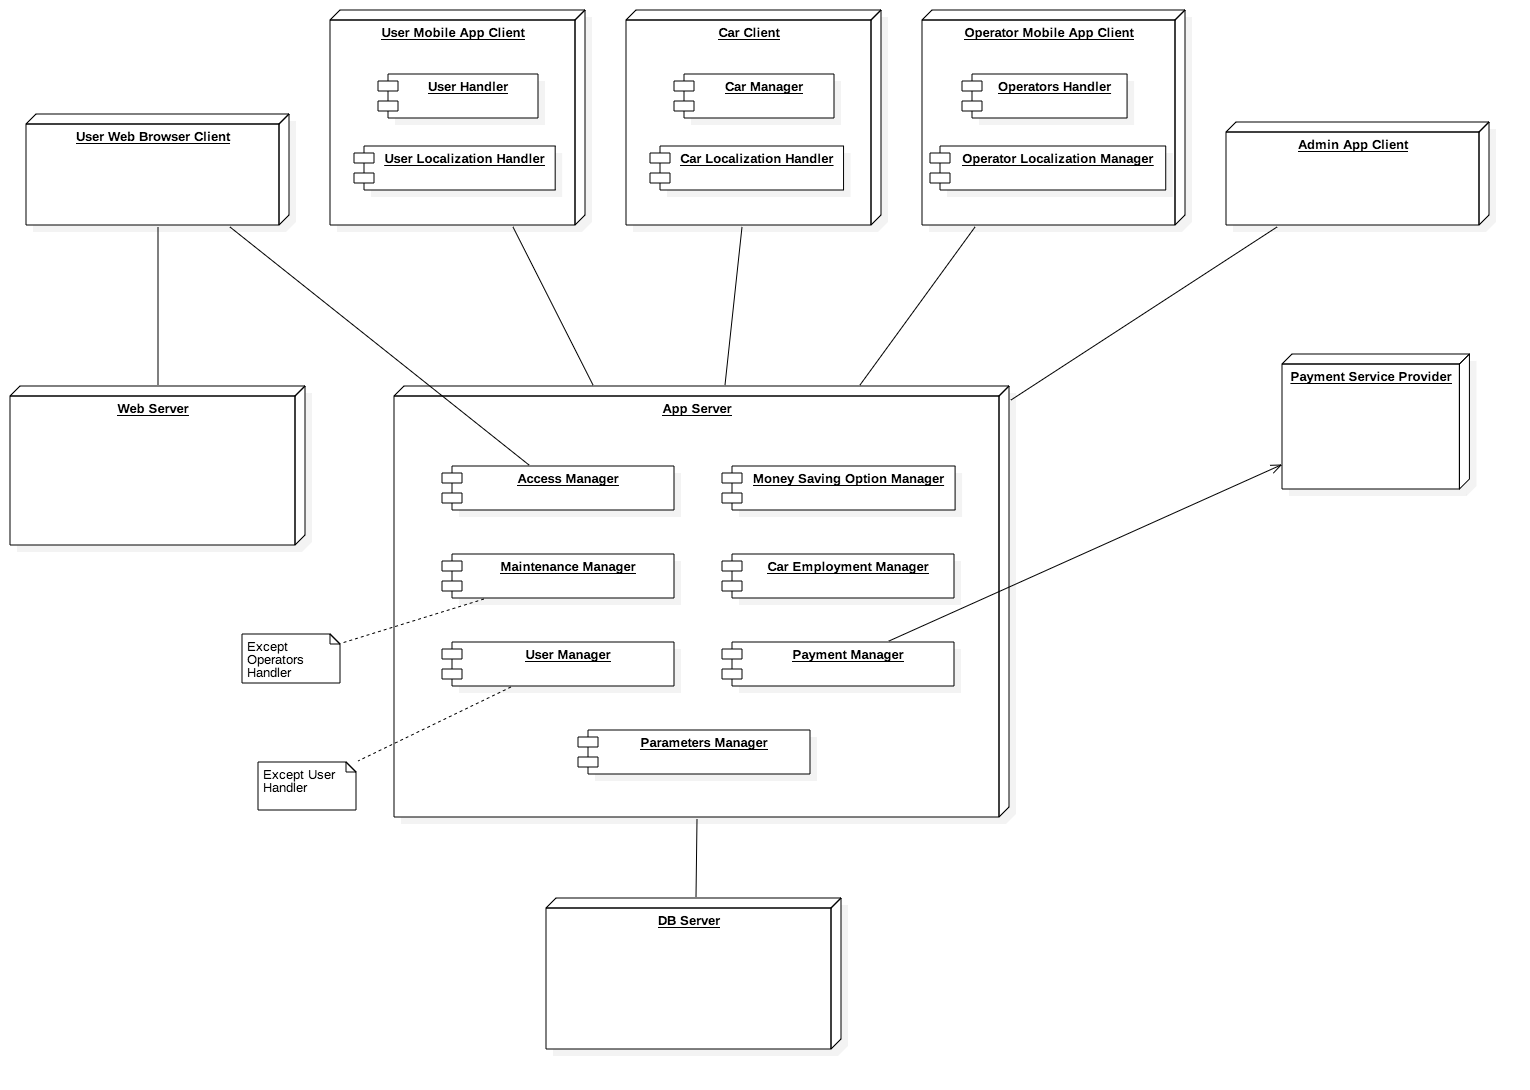
\includegraphics[width=\hsize, center]{img/deployment_diagrams/global.png}
	\caption{Logical deployment diagram: component allocation.}
\end{sidewaysfigure}

\subsubsection{Non-functional requirements choices}
	The architectural structure proposed addresses the non-functional requirements of \textit{integrity} and \textit{confidentiality} (see RASD) introducing a DMZ which separates with a firewall the app server, accessible from the outside network, from the database server. To avoid intrusions on the app server, another firewall is provided, with less restricting rules to allow outside clients to access. This way, even if an attack is performed to the app server, a more impenetrable layer of security still divides the intruders from the sensitive data. The structure just described is a standard pattern in the design of three-tier architectures.

	The app server is designed as a distributed system completely replicated in at least another physical machine, to fulfil the requirement of \textit{availabilty} and partially address the requirement of \textit{performance} (see RASD). A load balancer is expected to redirect the workload to the appropriate physical server. The number of servers can be increased in future if the workload requires it. This structure, along with a proper firewall configuration, helps to reduce the risk of failure for DOS attacks.

	Internally, each physical server is implemented following the \textit{elasticity pattern}, to fulfil the requirement of \textit{performance} (see RASD) while maintaining the number of allocated resources low. Thus, the components are to be instantiated according to the present load of clients' requests. An \textit{elastic load balancer} is used to manage the scaling process.

	To address the requirement of \textit{robustness} (see RASD) a simple error handling in the client application is enough. However, given the importance of failure management to avoid damages or theft to be performed to the cars, the data layer is chosen to be distributed.

	Lastly, the modularization of components and the possibility for the administrators to modify the core parameters of the system through the \textit{Parameters Manager} is conform to the \textit{design for flexibility} principle and satisfies the non-functional requirement of \textit{flexibility} (see RASD).
\FloatBarrier

\subsubsection{Technological choices}
	% TODO talk about technological choices for APIs, app server, db server, mobile apps, desktop apps, browser, ...
	From a technological point of view, the implementation of the system relies on the following choices.
	\begin{description}
		\item[User mobile app client.] The mobile app is to be developed with native technologies according to the mobile OS running on the device. In particular:
			\begin{description}
				\item[Android] Java for Android, with support for Android 4.4+.
				\item[iOS] Objective-C, with support for iOS 6+.
				\item[Windows Phone] C\#, with support for Windows 10 mobile.
			\end{description}
		The choice of covering the 3 most important OS on the market fulfils the \textit{design for portability} pattern. To address this pattern and be able to release the system in shorter time, some non-native options have been taken in consideration (e.g. Apache Cordova). However, this solutions showed to provide limited access to native functionalities such as the GPS system and the Bluetooth, which are instead very important for the system-to-be (i.e. localization, communication with the car). Therefore, native solutions have been preferred, to have full control of the device. This choice guarantees also a better user experience.

		\item[Operator mobile app client.] This internal application helps the operators to track their activity during the interventions. The company provides them with an Android tablet, so the application is to be compatible with it. Moreover, to provide more usability, this application is designed to be deployed on both tablet and smartphones, managing a responsive layout. The company choice of the Android platform addresses the need of inexpensive but efficient devices to run mainly the application. As for the \textit{User mobile app client}, the application is to be developed in native language (Java for Android, with support for Android 4.4+) to exploit some system-level functionalities.

		\item[Car client.] The system managing the whole car is running on the Android tablet installed. It is connected to the control unit of the car and communicates with the rest of the system though the APIs provided by the app server. It also exposes some APIs of its own, to be accessed by the app server (i.e. request of status information, sending of commands). Besides, a Bluetooth listener receives the requests from near users to unlock the car (if a reservation has been made).

		\item[Admin app client.] An internal desktop application is developed to provide access to the admin to the parameter manager and the operator dispatching area. To avoid restrictions in the future equipment of the admins, the application is planned to be developed in Java, ensuring portability on every desktop and laptop OS. In addition, given the configuration of the app server (see later), Java EE is required, to guarantee uniformity with the back-end system and simplify the development.

		\item[App server.] This server is to be developed using the Java EE platform. This framework will help to provide the elasticity required and simplify the connections with the database through JPA. The app server exposes the APIs required by the clients as RESTful web services.

		\item[Web server and User web browser client.] The web server simply hosts a very limited website with information about the service and an account management section. Given the simple functionalities, it is not worth the effort of building a Java EE system; instead, the most basic set of web technologies are to be used: HTML5, CSS3 and JS client-side and PHP7 server-side. The choice of PHP over other languages is due to the previous knowledge of the language by the team; in addition, it is a well spread language and can be easily maintained by other developers of the company in the future. For the account management section, the JS script communicates with the application server by means of AJAX calls to the web services.

		\item[Database server.] A distributed MySQL database, running on a set of Ubuntu servers, manages all the data needed by the application.
	\end{description}

\begin{sidewaysfigure}
	\includegraphics[width=\hsize, center]{img/deployment_diagrams/physical_deployment.png}
	\caption{Physical deployment diagram: technology choices and system distribution.}
\end{sidewaysfigure}

\FloatBarrier


		\subsection{Runtime view}
				
		\paragraph{} This section shows how the processes run and interact in the system. 
		We will present processes, that covers most features of our system: Login and Car Employment, which includes: Reservation of a car in specific zone, Picking up a reserved car, Riding a car. Employment of a car can be divided into several processes, but we decided to show them in one sequence diagram due to their close interaction.    

	\subsubsection{Login}	
		\begin{figure}[h]
			\includegraphics[scale=0.7]{img/LoginSD.png}
			\caption{Login sequence diagram }
		\end{figure}
		
		\paragraph{} This sequence diagram represents the User login. 
		The Guest has to fill the form on the Login page with his credential information and press Login as he's finished. 
		Then the Access Manager is notified that the Guest filled the form and wishes to log in, Access Manager sends this request to ProfileManagerl to check the data from the form and find it in the database. When the ProfileManager finishes the control of the data, there is to alternative scenarios of what will happen. 
		If the Guest has entered wrong data the Login form, the ProfileManager will send back to Access Manager a message, notifying that the given information was not found in the database, the error message will be displayed on the Login page. 
		If the Guest filled the form with right credentials, then the ProfileManager will confirm the Access Manager the correctness of the information, and the success message will be displayed on the Login Page, after which the Guest will redirected to User view.           
			
	\newpage
	\subsubsection{Car Employment}	
	
		\begin{figure}[h]
			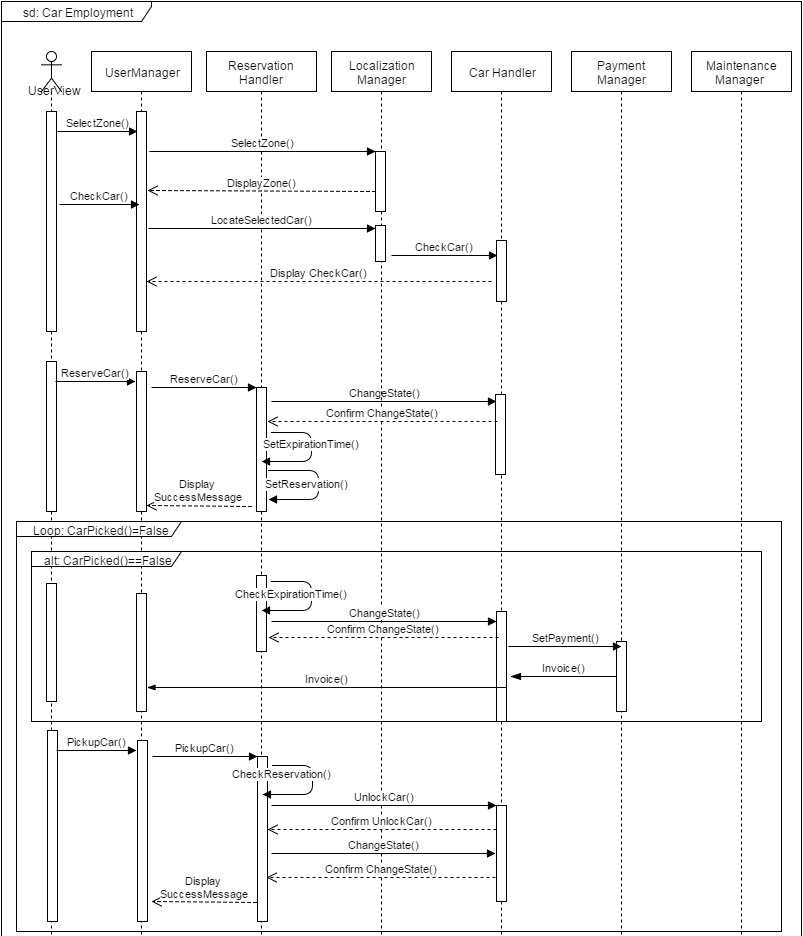
\includegraphics[scale=0.55]{img/CarEmploymentSD1.png}
			
		\end{figure}
		\newpage
		\begin{figure}[h]
			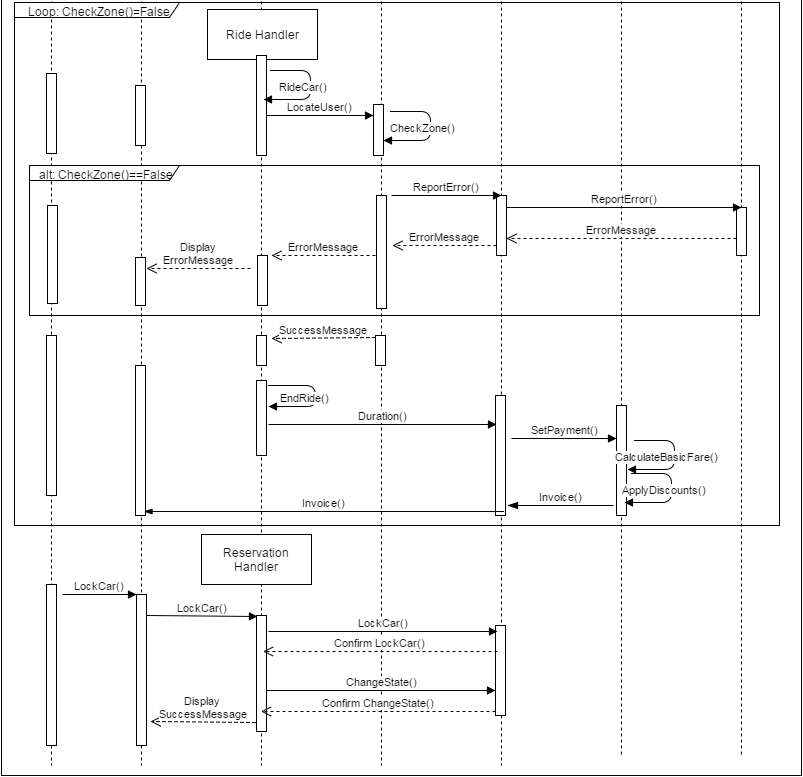
\includegraphics[scale=0.55]{img/CarEmploymentSD2.png}
			\caption{Car Employment sequence diagram}
		\end{figure}
		
		\paragraph{} This sequence diagram shows the employment of car by User.
		User selects the zone on the UserManager's interface in order to the system to understand the User's location, this information is sent to Localization Manager, which will save the selected zone, that will be displayed on the UserManager's interface. Now User can pick a car only from one specific zone. User selects a car on a UserManager's interface, the request is sent to Localization Manager, that gives detailed location of the car and sends request to check the car to Car Handler, which replies directly and the detailed information about the car is displayed. The User choses to reserve this car, the request is sent Reservation Handler that passes the request to Car Handler to change the state of the car to Unavailable. Car Handler answers back and confirms the change of car's state. The Reservation Handler sets the expiration time and registers the reservation, this will display as a message on the UserManager's interface. 
		
		After this procedure User has choice to pick up the reserved car or not.
		
		If by the expiration time the User will not pick up the car, the  Reservation Handler will send the request to Car Handler to change the state of the car back to Available, after the Car Handler gives confirmation of change of the state, it also notifies the Payment manager to set the payment (fee), Payment Manager gives back the invoice to Car Handler, then the user will be notified about the payment.   
		
		If the User picks up the reserved car on time, the request to pick up the car is sent to Reservation Handler, that checks the correctness of the reservation and sends the request to Car Handler to unlock the car and then to change the state of the car to In use, Car Handler confirms back both operations, this information is displayed on the UserManager's interface as success message.
		
		While the user rides the car, Ride Handler always keep in track with the location by sending the request to Localization Manager, that Check if the location is still in selected zone (if the car is still inside the city's boundaries). 
		
		If the User left the selected zone, Localization Manager reports the error to Car Handler, that passes it to Maintenance Manager, which replies back the error message, that goes to Localization Manager, Ride Handler and is displayed on the UserManager's interface.
		
		If the User is in the selected zone, then Localization Manager answers the Ride Handler with a success message.  
		
		The User ends the ride, this requests passes from UserManager's interface to Ride Handler, that sends request to Car Handler in order to check the car,   it confirms back with the information about the car. Car Handler sends the Payment Manager request to set the payment. Payment Manager calculates the basic fare, applies the discounts (if there are any) to the payment and sends invoice to Car Handler, the payment information notifies the User about the payment. 
		
		
		User Lock the car, this request is sent from UserManager's interface to Reservation Handler, that sends it to Car Handler and the car answers back with an confirmation. Reservation Handler sends request to Car Handler to change the state of the car to available, Car Handler answers back with confirmation that the state is changed, this information is displayed as success message.    


		\subsection{Component interfaces}
		\label{sec:components_interfaces}
				In this section we will show the component interfaces. Their main functions were already seen in the previous section, although there are basic parameters added for each. Nevertheless we need to keep in mind that for the further implementations, these functions can be splitted into less complex ones.  
		\newpage
		\begin{figure}[h]
			\includegraphics[scale=0.55]{img/Interfaces.png}
		\end{figure}


		\subsection{Selected  architectural  styles  and  patterns}
			
				
	\paragraph{} We decided that the architecture of our system has three tiers: the Presentation, that is provided by the interaction between the client and the Web Server, the Business Logic part is provided by the Server and the Persistence is provided by the Database that interacts with the Server.  	
	
	 In order to design and build our system we used several different strategies and patterns. Our systems is designed as an application and clients must be able to interact through the Internet, for this reason we used Client-Server architecture. Server can be achieved by several clients, it has easy maintenance, can be quickly replaced, repaired and upgraded, what's more, it has good security, where only authorized clients can access or manipulate data in the system. We also used the MVC pattern, where database acts as model, mobile application as view and the server as controller.  As it was mentioned before, another design logic we implemented is  cloud pattern (elasticity pattern), in order for the components to be instantiated according to current load of clients' requests. 
	
		

		\subsection{Other design decisions}
			\subsubsection{Database design}
	What follows is the class diagram representation of the database designed to store the data needed by the system. It embodies the data layer, and is stored by \textit{database servers}, which also provides access to it.\newline
	The reader will find comments on the diagram itself: they mainly reflect some constraint on the data represented, and are connected directly to the elements involved.\newline

	\begin{sidewaysfigure}
		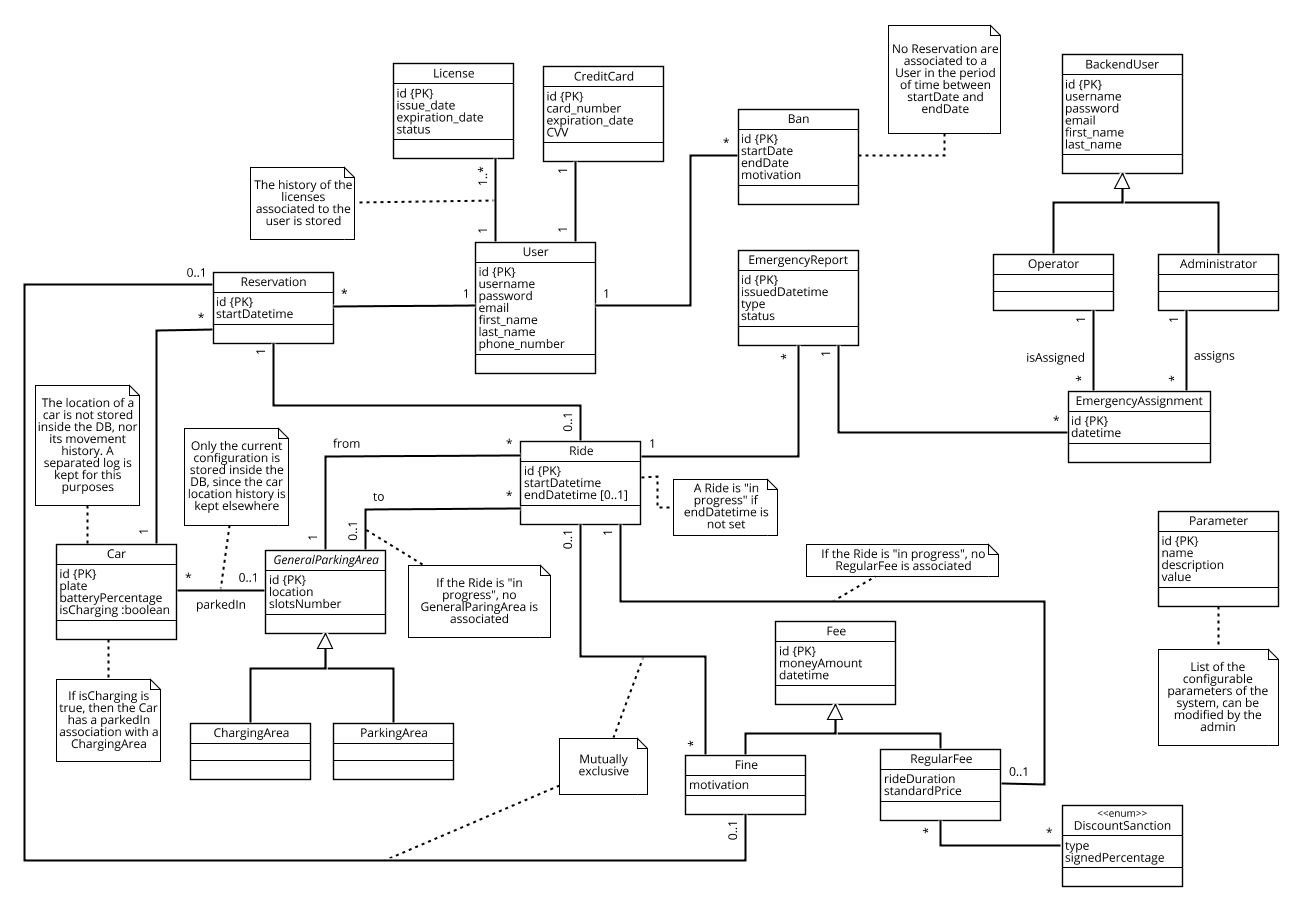
\includegraphics[width=\hsize, center]{img/db_class_diagram.png}
		\caption{Database design.}
	\end{sidewaysfigure}

	\noindent A clarification is needed, although a comment already summarizes it. The database stores the current state of the system as well as the history of its changes. The only exception to this policy is represented by the car location: given the high level of changes in the position of the car, due to its role in the system, it would be inefficient and resource-consuming to store all this information in a relational database. For this reason, a specific log - here not analysed - is introduced to keep track of the car movements and be able to retrieve them when needed (i.e. legal matters, theft, etc.).
\FloatBarrier


	\newpage
	\section{Algorithm design}
	\label{sec:algorithm_design}
		In this section we will describe the most interesting (from a computational point of view) algorithms; we have decided not to include algorithms for the more mechanical and common part of the system (such as login operations or interactions with the DBMS). Hence, the algorithms described in the following pages will be related to the calculation of the Money Saving Option component of the system.

\subsection{Money Saving Option algorithm}

\begin{algorithm}[H]
	\KwData{the destination given by the user}
	\KwResult{the area where to park to gain the money saving option discount}
	initialization\;
	
	$d\_location \leftarrow LocationServices.search\_location(destination)$\;
	$curr\_location \leftarrow LocationServices.search\_location(car)$\;
	$distance \leftarrow LocationServices.calculate\_distance (d\_location, curr\_location)$\;
	
	$starting\_battery \leftarrow getBattery(car)$\;
	$final\_battery\_estimate \leftarrow estimate(distance, starting\_battery)$\;
	
	$battery\_weight \leftarrow$ call on $battery\_importance\_algorithm(final\_battery\_estimate)$\;
	
	$list solutions(solution, delta) \leftarrow NULL$\;
	$list areas \leftarrow LocationServices.get($all parking areas within a 1km radius from $d\_location)$\;
	
	\ForAll{area in areas}{
		add car to area\;
		$delta\_availability \leftarrow$ call on $calculate\_solution\_quality\_algorithm(areas)$\;
		\If{area is $recharging\_area$}{$delta\_availability \leftarrow delta\_availability * battery\_weight$\;}
		$solutions \leftarrow insertByIncreasingDelta(area, delta\_availability)$\;
		remove car from area\;
	}
	
	$best\_solution \leftarrow solutions.getFirst$\;
	$notify\_car(best\_solution)$\;
	
	\caption{Money Saving Option}
\end{algorithm}

\paragraph{}The algorithm above describes the general idea behind the money saving option computation. For complexity reasons, we decided to keep the calculation of the best parking area within a limited radius of the user's destination. This also satisfies the need to choose an area in walking distance from the user's destination. 
Our assignment's request was that both the user's destination and the availability of power plugs be included in the choice of the safe area; the first one is taken into consideration when considering only a radius from the destination (we set it at 1km), while for the second one we created another algorithm: see the Battery Importance Algorithm section for further information on the battery weight.
The most important part of the algorithm is the evaluation of the quality of a solution. What we do is selecting the candidate areas to be the money saving option one (within the radius) and perform a cycle on them. For each area, we try to add the car to the area and evaluate the solution with the car added to that particular area (see the Solution Quality section for further information). We have a list of solutions (made of the area in which we have added the car in the particular solution and its quality measure) and for each cycle we add the new possible solution in decreasing order of quality (increasing order of delta). The quality measure is a double value between 0 and 1, representing a percent value. 
At the end of the cycle, we choose the area to tell the user by picking the first element of the solutions list: this means that it represents the best possible distribution of cars in the area, which means that parking the car in the given area will create the best possible distribution; however, not necessarily the one closer to the destination: that's why we need to keep the search confined to a limited area.
This algorithm's time complexity (without considering subroutines complexity) is linear in O(n), n being the considered number of areas.

\subsection{Solution Quality algorithm}

\begin{algorithm}
	\KwData{list of areas}
	\KwResult{a double value describing the quality of the solution}
	initialization\;
	$highest\_availability \leftarrow$ call on $calculate\_availability(areas.get(1))$\;
	$lowest\_availability \leftarrow highest\_availability$\;
	
	\For{i=2 to size of areas}{
		$availability \leftarrow$ call on $calculate\_availability(areas.get(i))$\;	
		\If{$availability >= highest\_availability$}{$highest\_availability \leftarrow availability$\;}
		\If{$availability >= lowest\_availability$}{$lowest\_availability \leftarrow availability$\;}
	}
	$delta \leftarrow highest\_availability - lowest\_availability$\;
	
	return delta\;
	\caption{Calculate Solution Quality}
\end{algorithm}

The solution quality algorithm stems from the assumption that we can define the quality of a distribution of cars as the difference (delta) between the maximum availability and the minimum availability of slots in the parking areas taken into consideration. Let's look at two examples to better understand this definition.
\paragraph{Example}In a specific zone of the city there are 5 areas. Let's say w.l.o.g. that they all have 10 parking slots; area 1 has 5 slots taken (i.e. an availability of 50\%), area 2 has 9 slots taken (i.e. availability=10\%), area 3 has 2 slots taken (i.e. availability=80\%), area 4 has 5 (availability=50\%), area 5 has 6 (availability=40\%). The delta of availability is 70\% (80\%-10\%).
In another zone on the other hand we have another 4 areas; regardless of how many cars versus free slots there are, let's say that area 1 has an availability of 30\%, area 2 an availability of 35\%, area 3 of 24\%, area 4 of 60\%. The delta of availability is 36\% (60\% - 24\%). This means that the second zone has a better distribution than the first one (even though there are less slots available).
\paragraph{}The delta is calculated by cycling through the list of areas and computing the maximum and minimum availability, and then by subtracting them. Notice that the time complexity of this algorithm is O(n), n being the size of the list of areas. This makes the whole money saving option algorithm (without considering the complexity requested to the external localization services provider for its own computations) quadratic in $O(n^2)$.

\begin{algorithm}
	\KwData{a parking area}
	\KwResult{a value between 0 and 1 representing the availability percent normalized}
	initialization\;
	$slots \leftarrow area.getDimentions()$\;
	$available\_slots \leftarrow area.getParkedCars().getSize()$\;
	$availability \leftarrow available\_slots / slots$\;
	
	return availability\;
	\caption{Calculate availability algorithm}
\end{algorithm}


\subsection{Battery Importance algorithm}
As the reader may have noticed, in the money saving option algorithm if the considered parking area is a recharging area the solution quality gets multiplied by a factor called $battery\_weight$, computed by passing the estimated final battery to a function called $battery\_importance\_algorithm$. 
The idea behind this adjustment of the solution's quality is that the lowest the car's battery is, the more important it is to park it in a recharging area; thus the solution's importance (i.e. its quality) is adjusted based on the battery of the car. 
We didn't write down the algorithm for this computation; instead we decided to work with a fuzzy model and write the specs for this system in FCL (fuzzy control language). The use of fuzzy logic is particularly useful for our system for two reasons: firstly, it's very simple to understand, and secondly it helps defining more realistic situations. In fact, since the battery is ideally a continuous value, the use of a boolean divide (e.g. If battery $<=50\%$ then apply the $battery\_weight$) would bring to a loss of richness in the system.
Below the reader will find the FCL code for our fuzzy model, with an explanation following.


\begin{verbatim}
FUNCTION_BLOCK

VAR_INPUT
    Battery      REAL; (* RANGE(0 .. 1) *) 
END_VAR

VAR_OUTPUT
    PlugImportance      REAL; (* RANGE(0,8 .. 1,5) *) 
END_VAR

FUZZIFY Battery
    TERM Very_Low := (0, 0) (0, 1) (0.2, 0) ;
    TERM Low := (0, 0) (0.2, 1) (0.5, 0) ;
    TERM Medium := (0.2, 0) (0.5, 1) (0.8, 0) ;
    TERM High := (0.5, 0) (0.8, 1) (1, 0) ;
    TERM Very_High := (0.8, 0) (1, 1) (1, 0) ;
END_FUZZIFY

FUZZUFY PlugImportance
    TERM Not_Important := 0.8;
    TERM Indifferent := 1;
    TERM Important := 1.2;
    TERM Very_Important := 1.4;
    TERM Fundamental := 1.5;
END_FUZZIFY


DEFUZZIFY valve 
    METHOD: CoG;
END_DEFUZZIFY

RULEBLOCK batteryWeight
    ACCUM:MAX;

    RULE 0: IF (Battery IS Very_High) THEN (PlugImportance IS Not_Important);
    RULE 1: IF (Battery IS High) THEN (PlugImportance IS Indifferent);
    RULE 2: IF (Battery IS Medium) THEN (PlugImportance IS Important);
    RULE 3: IF (Battery IS Low) THEN (PlugImportance IS Very_Important);
    RULE 4: IF (Battery IS Very_Low) THEN (PlugImportance IS Fundamental);
END_RULEBLOCK

END_FUNCTION_BLOCK
\end{verbatim}

\paragraph{} Fuzzy models are based on the idea that objects not necessarily belong completely inside a set or outside of it; hence, fuzzy logic does not assign a boolean value to the membership function of an element (i.e. if an element is a member of a set) but instead a real value between 0 and 1. In our case, we thought simplicistic to think of the battery either as "empty" (boolean value 0) or "full" (boolean value 1) if above or below 50\%, so we decided to describe it with a fuzzy variable called Battery. This input variable has range $[0, 1]$ and five labels that describe it: very low, low, medium, high, very high. The same reasoning is applied to the variable PlugImportance, which will later be returned to the caller as the $battery\_weight$. Notice that the variable PlugImportance has discrete values between 0.8 and 1.5: colloquially, if the battery is not important then its weight is 0.8 (less than 1) and the quality of a solution where the car is parked in a recharging area lessens. On the other extreme of the spectrum, if the battery is very important (i.e. there's no charge left) then it's fundamental to put the car in a recharging area, thus the quality of a solution where the car is parked in a recharging area increases by 1.5.
This informal reasoning is formalized in the block of code called \textit{RULEBLOCK}: these rules represent the relationship between the input value and the output. 
The defuzzyfying method is CoG, i.e. Center of Gravity (Centroid), which calculates the center of the area of the fuzzy set and uses the value at which this occurs as the defuzzified output.

	\newpage
	\section{User interface design}
	\label{sec:user_interface_design}
		This section provides mockups and general descriptions on the UI of the different client applications.

\subsection{User web browser client}
	% TODO see RASD

\subsection{User mobile app client}
	% TODO see RASD

\subsection{Car client}
	% TODO

\subsection{Operator mobile client}
	% TODO

\subsection{Admin app client}
	% TODO


	\newpage
	\section{Requirements traceability}
		What follows is a list of the requirements for the system defined in the RASD and an explanation about how the design exposed in this document fulfils them. The explanation will be in italics, following the points it is referring at.

\begin{itemize}
\item \textit{G[1]} The system allows guests to register; to complete the registration procedure the system sends a password to the guest as an access key.

	\textit{The website and the mobile application allow any guest to register into the system.}

	\begin{itemize}
		\item R[1.1] The system has to allow any person to submit only one account request.
		\item R[1.2] The system must accept an account request only if the credit card owner's name and the user's name coincide.
		\item R[1.3] The account is created when an admin validates all the necessary data.

			\textit{The uniqueness of the accounts are granted by the manual check performed by the admin before confirming a user's registration (see RASD for further explanations). They also validate the inserted data, included the credit card information.}

		\item R[1.4] The system must be able to generate passwords.
		\item R[1.5] The system has to send a newly generated password to the user via email when the account is created.
		\item R[1.6] The system must be able to check whether a password is correct or not.
		\item R[1.7] The system must let the user log in only if the password is correct. 
		\item R[1.8] The system has to generate a new password and send it via email if the user asks for it.

			\textit{All the previous operations are managed by the Access Manager component.}
	\end{itemize}

\item \textit{G[2]} The system should enable a registered user to find the location of an available car within a certain distance from the user's location or from a specified address.

	\textit{One section of the mobile application is dedicated to the lookup of cars near the current location or an address. The Localization Manager component takes care of the location retrieval and management, while the Parking Manager and the Car Manager are responsible for finding the available cars.}

	\begin{itemize}
		\item R[2.1] The system must have the ability to locate the user if the user's GPS is on.
		\item R[2.2] The system is able to locate any valid address.
		\item R[2.3] The system is able to find any of the parking areas of the company.
		\item R[2.4] The system is able to identify available cars inside parking areas. % XXX is it done by gps or some strange technology we haven't named anywhere? in latter case, this may be said, here and somewhere else

			\textit{The Location Service Provider assures to be able to locate any valid address inside the city. Besides, the addresses of every parking area are known by the system and used to localize them.}

		\item R[2.5] The system lets users see whether there are available cars in a specified radius.

			\textit{The cooperation of the components previously mentioned allows the system to display the available cars in a map, setting a distance constraint.}
	\end{itemize}
	
\item \textit{G[3]} The system enables user to reserve a single available car in a certain geographical region for one hour before the user picks it up. If the car is not picked up by that time, the reservation expires, the system tags this car as available again and it charges the user a fine of 1 EUR.

	\textit{The Reservation Manager is responsible for managing the reservation of a car. Cooperating with the Time Manager for the time tracking activities, it also communicates any possible expiration to the Exceptional Payment Manager component to apply an appropriate fee to the user.}

	\begin{itemize}
		\item R[3.1] The system allows users to reserve an available car.

			\textit{This is the main functionality of the Reservation Manager.}
		
		\item R[3.2] The cars cannot be reserved by more than one user at any given time.

			\textit{The database structure does not allow a reservation of a car by more than one user in the same moment.}

		\item R[3.3] The system keeps the current reservation standing until the user has opened the car or an hour has passed.
		\item R[3.4] The system autonomously cancels a reservation if the user who has reserved it hasn't picked it up after one hour.

			\textit{The Time Manager is able to keep track of the time passed and inform the Reservation Manager of the expiration. If the user opens the car within the hour, the Time Manager is informed and the count stops. The expiration triggers the additional fees on one side, and the reservation annulment on the other.}

		\item R[3.5] The system must impede any user with an expired license to reserve a car.
		\item R[3.6] The system must impede any banned user to reserve a car.

			\textit{The Reservation Manager performs this checks before confirming the operation.}
	\end{itemize}

\item \textit{G[4]} The system should allow the user to employ a car in a proper and safe way. 

	\textit{The mobile application and tablet installed on the car keep the user informed about the current ride and are able to provide him additional information when needed. The Car Employment is the component most responsible for these operations.}

	\begin{itemize}
		\item R[4.1] The system must be able to locate any car at any given time. 
		\item R[4.2] The system detects whether there are passengers inside a car, and how many.
		\item R[4.3] The system must be able to collect data about the power charge of any of its cars.
		\item R[4.4] The system detects when a severe accident has occurred to a car.
		\item R[4.5] The system must be able to detect when a user is near a car.
		\item R[4.6] The system must be able to tell when a car is parked in a safe area.
		\item R[4.7] The system must be able to detect when a car is plugged to the power grid.
		\item R[4.8] The system must be able to detect whether the driver is still in the car.

			\textit{All the previous requirements are satisfied by the construction of the car and its sensors equipment (see RASD).}

		\item R[4.9] The system automatically unlocks a car when the user that has reserved is nearby.
		\item R[4.10] The system automatically locks a car when the user has exited it inside a safe area. 
		\item R[4.11] The system allows the user to lock and unlock their car manually when outside a safe area.

			\textit{The interaction between the Car Manager and the User Manager leads this operations to be put into effect. Notice that a car can notice the proximity of a user using its Bluetooth equipment, given that the user allows it to do so from the mobile application.}

		\item R[4.12] The system provides a finite time window that begins when the user exits the car inside a safe area. The time window must either end when the allotted time is finished or when another user reserves the same car.
		\item R[4.13] The system allows the user to re-enter the car if the time window is still open and the user tries to manually open it.

			\textit{The Time Manager deals with the time windows, while the rest of the Car Employment component covers what is left.}
	\end{itemize}
	
\item \textit{G[5]} The system charges the user for a predefined amount of money per minute. A screen on the car notifies the user of the current charges.

	\textit{Both the car tablet and the mobile application provide information about the current ride, including the current charges. The charges are computed by the Payment Manager component and sent to the Payment Service Provider to be made effective.}

	\begin{itemize}
		\item R[5.1] The system is able to retrieve all data necessary to charge the user. This data is the duration of the ride and all the conditions for the eventual application of discounts and sanctions.
		\item R[5.2] The system notifies the user of the fee per minute he's being charged through a screen inside the car.
		\item R[5.3] The system notifies the final charges to the user after the time window for the ride has expired.
		\item R[5.4] The system invoices the user after the time window for the ride by communicating the charges to the external payment system. 
		
	\end{itemize}

\item \textit{G[6]} The system starts charging the user as soon as the car ignites. It stops charging them when the car is parked in a safe area and the user exits the car.

	\textit{The Car Employment component addresses this requirement communicating mainly with the Car Manager, to retrieve information about the sensors and the car status.}

	\begin{itemize}
		\item R[6.1] The system charges the user with a fee per minute.
		\item R[6.2] The system can tell when the car has ignited. 
		\item R[6.3] The system stops counting the charges for a standard ride when the user exits the car while inside a safe area.
		\item R[6.4] The system starts charging the user when the car ignites or when the reservation expires while the user is inside the car.
	\end{itemize}
	
\item \textit{G[7]} The system should encourage good user behaviour through the application of discounts to the fee per minute.

	\textit{The Discount and Sanction Handler is responsible for this computation.}

	\begin{itemize}
		\item R[7.1] The system applies all discounts to the fee per minute.
		\item R[7.2] If the conditions for a discount are satisfied only for a limited period of time during the ride, the discount is applied only to that time period.
		\item R[7.3] The system applies a discount every time a user brings two or more passengers in the car with them and the car is on.
		\item R[7.4] The system applies a discount to the total fee for the ride when the car has more than 50\% of power charge by the end of a standard ride.
		\item R[7.5] The system applies a discount to the total fee for the ride every time the car for that ride is plugged to the power grid at the end of the time window. 
		\item R[7.6] The system calculates the total discount as the sum of the singular discounts applied to the ride. If this sum exceeds 100\%, then it is considered simply as 100\%.

			\textit{Notice that to accomplish these tasks some information from the car is required, and it is actually retrieved by the Ride Handler component, directly connected with the Discount and Sanction Handler. }
	\end{itemize}
	
\item \textit{G[8]} The system should discourage bad behaviour through the application of sanctions to the fee per minute.

	\textit{The Discount and Sanction Handler is responsible for this computation.}

	\begin{itemize}
		\item R[8.1] The system applies a sanction every time a car is returned in a safe area at more than 3 km from the nearest recharging safe area.
		\item R[8.2] The system applies a sanction every time a car is returned with less than 20\% of power charge.

			\textit{Notice that, as for G[7], to accomplish these tasks some information from the car is required, and it is actually retrieved by the Ride Handler component, directly connected with the Discount and Sanction Handler. }
	\end{itemize}
	
\item \textit{G[9]} The system provides an alternative usage mode for cars called \textit{money saving option}. Besides aiding the user in saving money, this mode allows for a uniform distribution of cars throughout the city by suggesting the user where to park.

	\textit{An apposite component (Money Saving Option Manager) is reserved for these computations.}

	\begin{itemize}
		\item R[9.1] The system allows a user to select the \textit{money saving option} at any point during their ride.

			\textit{The money saving option can be activated from the mobile application and from the car tablet, as shown in \autoref{sec:user_interface_design}.}

		\item R[9.2] The system applies a discount every time the car is returned in the suggested safe area with the \textit{money saving} option.

			\textit{This is addressed by the Payment Manager component, interacting with the Car Employment component.}

		\item R[9.3] The system selects the safe area suggested to the user through the available algorithm. (see text assumptions)

			\textit{The algorithm proposed in \autoref{sec:algorithm_design} has been designed to achieve a uniform distribution and a dependence from the presence of power plugs, as requested by the clients and expressed in the RASD.}

	\end{itemize}
	
\item \textit{G[10]} The system allows the company to assist the users in case of need and take care of the cars.

	\textit{The position of operator has been introduced to provide assistance to the users. They are equipped with a tablet and the operator's mobile application has been designed to help them.}

	\begin{itemize}
		\item R[10.1] The system allows a user to notify the back-end administrators if they have a problem with the car.
		\item R[10.2] The user must specify whether this problem is an accident or a reparation.

			\textit{The mobile application and the car tablet application allow the user to open an emergency report, specifying the type of emergency and adding a short description, as shown in \autoref{sec:user_interface_design}.}

		\item R[10.3] The system can locate \textit{PowerEnJoy} operators. 
		\item R[10.4] The system allows administrators to know the status of on-site operators and dispatch them if they are available.

			\textit{Every operator is equipped with a tablet running an apposite application. This allows them to communicate with the administrators and to be located. The admin application is provided with a section for the emergency reports management (see \autoref{sec:user_interface_design}), which main functionality is the dispatch of operators.}

		\item R[10.5] The system keeps track of every car's battery and alerts the admin when it lowers below 3\%. 
		\item R[10.6] The system notifies the admin when it detects that an accident occurred.

			\textit{The car system is equipped by construction to achieve this purposes by means of its sensors. The car tablet collects the information and sends it to the app server.}

		\item R[10.7] If the system has already notified the admin of an accident, then it must prevent the user from notifying it again.
		\item R[10.8] If the system has already notified the admin of an accident, then it must notify the user of this fact.
		\item R[10.9] Every time the system detects or a user notifies a problem, an emergency report is opened.

			\textit{The database structure helps managing the uniqueness of the reports. Moreover, the application server manages the notifications to the users.}

		\item R[10.10] Operators can change an emergency report status only when they are assigned to it.
		\item R[10.11] The system considers all type of emergency reports related to a reparation as on-site at first.
		\item R[10.12] The system allows operators to change the type of emergency reports related to a reparation from on-site to not on-site.
		\item R[10.13] Operators can change the type of emergency report from accident to reparation or vice versa only if they are assigned to it.

			\textit{Using the designated mobile application, operators can modify the status of an intervention and communicate it to the administrators. The constraints on the status and type of the emergency reports are managed by the Maintenance Manager, as well as the logic related to them.}
	\end{itemize}
	
\item \textit{G[11]} The admin should be able to configure some parameters of the system.

	\textit{The admin application addresses this goal providing a section for the configuration of the main parameters of the system.}

	\begin{itemize}
		\item R[11.1] The system allows the aministrators to modify parameters that influence the usage of cars. This parameters are:
			\begin{enumerate}
				\item The standard fee per minute
				\item The lost reservation fee (starting value = 1EUR)
				\item The time before considering a reservation lost (starting value = 1 hour)
				\item The fine for leaving an accident site
				\item Discount percent   values:
					\begin{itemize}
						\item Passengers discount (starting value = 10\%)
						\item Residual battery discount (starting value = 20\%)
						\item Plugged car (starting value = 30\%)
						\item Money saving option (starting value not defined)
					\end{itemize}
				\item Sanction percent values:
					\begin{itemize}
						\item Residual battery sanction (starting value = 30\%)
						\item Distance from power grid sanction (starting value = 30\%)
					\end{itemize}
				\item Time window for reservation fee
				\item Time window after ending the ride for reopening and pluggin the car.
				\item The fine for unnecessary emergency request.
			\end{enumerate}
	\end{itemize}
\end{itemize}

% TODO add non-funct req explaination (maybe refer to deployment section)


	\newpage
	\section{Effort spent}
		\begin{description}
			\item[Abbud, Patricia] around 36 hours of work;
			\item[Andreoli Andreoni, Maddalena] around 39 hours of work;
			\item[Cudrano, Paolo] around 53 hours of work.
		\end{description}

	\newpage
	\section{References}
		\subsection{Used tools}
		\begin{description}
			\item [LaTeX] The group used LaTeX to structure the final document and to help with versioning.
			\item [Github] We leaned on Github for versioning and coordinating synchronized work.
			\item [Toggl] We used toggl to keep track of work hours.
			\item [Slack] We used Slack for messaging and coordinating between us.
			\item [StarUML, Draw.io and Signavio] We used StarUML, Draw.io and Signavio as online and offline tools to draw UML diagrams and high-level diagrams.
			\item [Balsamiq] We used Balsamiq for the mockups.
		\end{description}
	
	\section{Changelog}
	From version 1 to version 2 we:
		\begin{itemize}
			\item Fixed some dependencies in Component View: added dependency between Car Location Handler and Reservation Handler, changed direction of the Admin Handler dependencies and Car Handler dependency.
			\item Enriched and completed interfaces diagram.
			\item Fixed some discrepancies in Sequence Diagram.
		\end{itemize}			
	
	\newpage
	\section{Appendix}
	\listoffigures

\end{document}
